\documentclass{article}                                                                           %basic LaTeX document type

\usepackage[margin=1.3in]{geometry}                                                     %set size of all margins
%\usepackage[left=1.3in, top=1in, right=1in, bottom=1in]{geometry}         %can set margin sizes which are not the same in this way

%\linespread{2}                                                                                         %option 1 for making text double-spaced
\usepackage{setspace}                                                                             %option 2 for making text double-spaced
\doublespacing                                                                                         %set double space

\usepackage{indentfirst}                                                                          %makes first paragraph of section indented (non-first are by default)
\setlength{\parindent}{25pt}                                                                     %set size of indentation (15pt is default)

\renewcommand\thesection{\Roman{section}}                                         %set capital Roman numeral section headings
\renewcommand\thesubsection{\thesection.\Alph{subsection}}                   %set capital Aramaic letters subsection headings
\renewcommand\thesubsubsection{\thesubsection.\arabic{subsubsection}} %set capital Arabic numbers subsubsection headings

\renewcommand*\thetable{\Roman{table}}                                              %set capital Roman numeral table numeration

\usepackage[explicit]{titlesec}                                                                  %package needed for next lines
\titleformat{\section}{\bfseries}{\thesection.}{1em}{\MakeUppercase{#1}}  %makes section headings bold and upper case characters
\titleformat{\subsection}{\bfseries}{\thesubsection.}{1em}{#1}                   %makes subsection headings bold
\titleformat{\subsubsection}{\itshape}{\thesubsubsection.}{1em}{#1}          %makes subsubsection headings in italics

\usepackage{lastpage}                                                                             %package which returns number of last page (same as number of pages)
\usepackage[figure,table]{totalcount}                                                        %package which counts the number of tables and/or figures

\usepackage{amsmath}                                                                            %enable `align' equation types

\renewcommand{\thefootnote}{\alph{footnote}}                                        %sets labeling of footnotes
\usepackage[]{footmisc}                                                                          %enables double spaced footnotes
  \renewcommand{\footnotelayout}{\doublespacing}                                  %double spacing of footnotes

%%% If you desire to place footnotes at the end of the document, uncomment these four lines and the two related near the end of this file
%\usepackage{endnotes}                                                                          %enables endnote page
%  \let\footnote=\endnote                                                                         %sets footnotes to endnotes
%  \renewcommand*{\theendnote}{\alph{endnote}}                                   %labels endnotes alphabetically
%  \renewcommand{\notesname}{Footnotes}                                            %renames endnotes title to footnotes

\usepackage{graphicx}                                                                             %enable figures
\usepackage{multirow}                                                                             %enable `multirow' capability in tables

\usepackage{caption}                                                                              %enables subfigures
\usepackage[labelformat=simple]{subcaption}                                           %enables subfigure captions 
\captionsetup[table]{labelsep=newline,name=TABLE}                                 %sets table caption formatting options to meet NSE requirements
\captionsetup[figure]{name=Fig.,labelsep=period}                                     %sets figure caption options to meet NSE requirements
\renewcommand*\thesubfigure{(\alph{subfigure})}                                    %enables proper labeling of subfigures

\usepackage[colorlinks=true, allcolors=blue]{hyperref}                               %reference and citation hyperlinking linking

\DeclareMathOperator{\diff}{d}                                                                %can define operators to use in math mode, example in Eq. 2
\DeclareMathOperator{\erf}{erf}

\begin{document}

%Define fields for \maketitle

\title{{\LaTeX} Template for Submissions to \\American Nuclear Society Journals} %title of paper

\author{
\vspace{20mm}
\\Aaron J. Olson,$^{\text{a},\ast}$ Mario I. Ortega,$^{\text{a,b}}$ and Eric M. Benner$^\text{c}$ \\[4pt] %list of authors, with corresponding author marked by asterisk
\textit{$^a$Sandia National Laboratories, Radiation Effects Theory Department}\\[-10pt]       %affiliations of authors
\textit{P.O. Box 5800, MS1179, Albuquerque, New Mexico 87185} \\[-5pt]
\textit{$^b$University of California Berkeley, Nuclear Engineering Department} \\ [-10pt]
\textit{4155 Etcheverry Hall, MC 1730} \\ [-10pt]
\textit{University of California, Berkeley, Berkeley, CA 94720-1730} \\ [-5pt]
\textit{$^c$University of New Mexico, Chemical and Biological Engineering Department} \\ [-10pt]
\textit{MSC01 1120, 1 University of New Mexico, Albuquerque, New Mexico 87131} \\ [-2pt]
{$^\ast$Email: \href{mailto:aolson@sandia.gov}{aolson@sandia.gov}}}       % email address for correspondence

\date{                               %instead of returning the date, this repurposes the \maketitle command to print the number of pages, tables, and figures
\vspace{40mm}
Number of pages: \pageref*{LastPage} \\
Number of tables: \totaltables \\
Number of figures: \totalfigures
}

\clearpage\maketitle
\thispagestyle{empty}


\pagebreak
~\vfill

\begin{abstract}
Having an appropriate {\LaTeX} template available when writing new papers saves authors time and effort.
As of the summer of 2017, the American Nuclear Society (ANS) had not had a {\LaTeX} template for submissions to their three journals: Nuclear Science and Engineering (NSE), Nuclear Technology (NT), and Fusion Science and Technology (FST).
While such a template may have existed in one or more forms and enjoyed use in a subset of the nuclear engineering community, asking colleagues did not yield knowledge of such a template.
We therefore asked the ANS editors if they would be interested in such a template, iterated with them to create one which was in agreement with the journal submission guidelines, and have provided it for the journal community to use.
Submissions need not strictly adhere to a specific form beyond what is specified in the submission guidelines since ANS will reformat accepted submissions for publication, we expect that this template will speed up the publishing process for researchers working with ANS.

\vspace{1em}\noindent\textbf{Keywords} --- ANS journal guidelines, ANS submission template, ANS bibliography style
\end{abstract}

\vfill


\pagebreak
\section{Introduction}

The usefulness of a template is increased if examples are given of many things that an author may encounter.
For example, the introduction to the paper goes here in the first section.
Let's use this introduction as a chance to cite different types of references including a book~\cite{Pomraning1991book}, a non-ANS-produced journal paper~\cite{AdamsJQSRT1989}, an ANS transactions paper~\cite{ZimmermanANS1991}, an ANS-produced journal paper~\cite{DonovanNSE2003}, a master's thesis~\cite{Vasques2005thesis}, a dissertation~\cite{Fichtl2009dissertation}, a conference paper~\cite{BrantleyMC2009Incident}, and a national laboratory report~\cite{PautzSAND2017AMClosurePres}.
These publications have been selected to demonstrate how to cite different types of works---not to provide an exhaustive introduction to the stochastic media problem in radiation transport.\footnote{Some of these references have more mature counterparts, e.g., Ref.~\cite{BrantleyMC2009Incident} is a conference paper whose content is encompassed by and expanded on in a journal paper.}

A seminal book on the problem of radiation transport in stochastic media was published in the early 1990s~\cite{Pomraning1991book}.
This body of work yielded a highly referenced journal paper presenting the ``Levermore--Pomraning'' (LP) closure~\cite{AdamsJQSRT1989}.
Soon thereafter a Monte Carlo algorithm was proposed by Zimmerman and Adams (Ref.~\cite{ZimmermanANS1991}) which has been shown to produce results equivalent to those given by the LP closure, as well as an algorithm that is usually more accurate.
Various extensions to these Monte Carlo algorithms have been investigated including variants intended for use with non-Markovian media~\cite{DonovanNSE2003}.
Work on this topic has continued, including in the academic realm, yielding a master's thesis which was a review of the dominant methods at that time~\cite{Vasques2005thesis} and a dissertation investigating an entirely new approach~\cite{Fichtl2009dissertation}.
One outcome of a newer body of work was to produce Monte-Carlo-based benchmarks~\cite{BrantleyMC2009Incident}.
Researchers continue to develop new approaches to solving transport results in stochastic media problems, as evidenced by Ref.~\cite{PautzSAND2017AMClosurePres} (a corresponding conference paper exists).

The next section details the use of equations, while Sec.~\ref{sec:tables} provides examples of table usage.
Secs.~\ref{sec:figures} and~\ref{sec:sections} contain example usages of figures and subheadings, respectively.
We conclude with a link to the ANS submission guidelines in Sec.~\ref{sec:conclusion}.



\section{Equations}
\label{sec:equations}

Equations are a part of the grammatical syntax of a sentence and may be a vital part of an independent clause; Eq.~(\ref{eqn:chordlength}) provides an example of this.
Ref.~\cite{AdamsJQSRT1989} explains that in binary Markovian media, the probability of finding material \(i\) at any point in the rod is given by
\begin{equation}
  p_i = \frac{\lambda_i}{\lambda_0 + \lambda_1}.
  \label{eqn:chordlength}
\end{equation}
Equations may also be a parenthetical statement to further explain the meaning of a sentence but are not required to form an independent clause.
This sentence and the following equation, which states the Levermore--Pomraning equations as written in Ref.~\cite{AdamsJQSRT1989}, provides an example:
\begin{align}
\begin{split}
  v \frac{\partial(p_i \psi_i)}{\partial t} + \Omega \nabla(p_i \psi_i) + \sigma_i p_i \psi_i &= \left[ \frac{\sigma_{si}}{4\pi} \right] \int_{4\pi} \diff \Omega' p_i \psi_i(\Omega') + p_i S_i + \frac{p_j \psi_j}{\lambda_j} - \frac{p_i \psi_i}{\lambda_i}, \\ 
  & i, j = 0,1, \qquad j \neq i.
\end{split}
  \label{eqn:LPequations}
\end{align}



\section{Tables}
\label{sec:tables}

Tables ought to be formatted to span either one or two columns and referenced specifically in the text.
For example, Tables~\ref{tab:params} and~\ref{tab:results}, based off of tables in Ref.~\cite{BrantleyMC2009Incident}, describe the input parameters and some numerical results for benchmark cases first presented in Ref.~\cite{AdamsJQSRT1989}.
Table~\ref{tab:params} is an example of a one-column table, and Table~\ref{tab:results} is an example of a two-column table.

\begin{table}%[!htbp]
\centering
\caption{Benchmark Set Parameters}
\label{tab:params}
\begin{tabular}{|ccccc|}
\hline
    Case & \(\Sigma_{t,0}\) & \(\Sigma_{t,1}\) & \(p_0\) & \(\lambda_c\) \\ \hline
    1               & 10/99 & 100/11 & 0.9 & 0.099\\
    2               & 10/99 & 99/10   & 0.9 & 0.99 \\
    3               & 2/101 & 200/101  & 0.5 & 2.525 \\ \hline
\hline
    Case  & $c_0$ & $c_1$ &  \multicolumn{2}{|c|}{Slab Thickness}  \\ \hline
    a               & 0.0 & 1.0 & \multicolumn{1}{|c}{\(L=\)} & 0.1 \\
    b               & 1.0 & 0.0 & \multicolumn{1}{|c}{\(L=\)} & 1.0 \\
    c               & 0.9 & 0.9 & \multicolumn{1}{|c}{\(L=\)} & 10.0 \\ \hline
\end{tabular}
\end{table}

\begin{table}[b]%[!htbp]
\centering
\caption{Reflection and Transmission Probability Comparisons}
\label{tab:results}
\begin{tabular}{|c|c|c|c|c|c|c|c|}
\hline
            &         &              &                 &                   &                  & \multicolumn{2}{c|}{Relative Error $E_{\langle R \rangle,\langle T \rangle}$} \\\hline
    \(L\)   & Case & Quantity & Benchmark & Algorithm A & Algorithm B & Algorithm A & Algorithm B \\ \hline \hline
    \multirow{4}{*}{0.1}   & \multirow{2}{*}{a} & \(\langle R \rangle\) & 0.04864 & 0.04768 & 0.04876 & -0.020 & 0.002 \\
                                     &                              & \(\langle T \rangle\) & 0.93650 & 0.93463 & 0.93350 & -0.002 & -0.003 \\ \cline{2-8}
                                     & \multirow{2}{*}{b} & \(\langle R \rangle\) & 0.00868 & 0.00847 & 0.00860 & -0.024 & -0.009 \\
                                     &                              & \(\langle T \rangle\) & 0.90432 & 0.90062 & 0.90080 & -0.004 & -0.004 \\ \hline
\end{tabular}
\end{table}



\section{Figures}
\label{sec:figures}

Like tables, a figure may also span one column or two.
All figures in this template were produced by taking screenshots of figures in cited works and saving them to \texttt{png} format and do not always meet line and caption requirements.
Additionally, figure widths here are suppressed to enable the larger page margins for submission documents.
Submitted figures should be in formats such as \texttt{tiff}, \texttt{eps}, or \texttt{pdf} and meet letter and line size requirements when the appropriate widths for the final version are used.

\begin{figure}[t]%[!htbp]
  \centering
  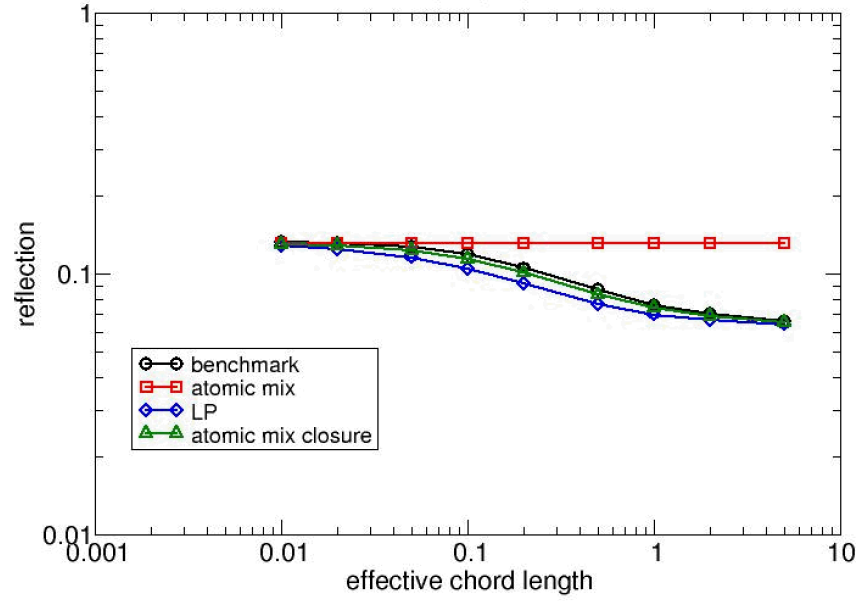
\includegraphics[trim = 10mm 0mm 15mm 15mm, width=70mm]{AMClosure.PNG}
  \caption{Reflection computed using four different methods as a function of effective chord length.}
  \label{fig:AMClosure}
\end{figure}

\begin{figure}%[!htbp]
  \centering
  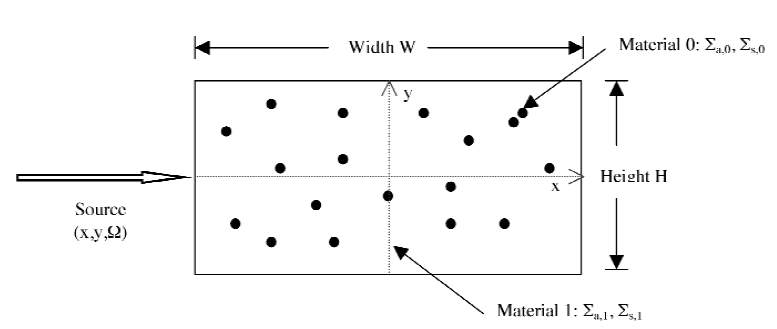
\includegraphics[trim = 10mm 0mm 10mm 0mm, width=140mm]{DonovanFig1.PNG}
  \caption{Binary stochastic mixture: disks embedded in a matrix; $\Sigma_{a,i}$ is the absorption coefficient of material $i$ (cm$^{-1}$), and $\Sigma_{s,i}$ is the scattering coefficient of material $i$ (cm$^{-1}$).}
  \label{fig:DonovanFig1}
\end{figure}

\begin{figure}%[!htbp]
  \centering
  \begin{subfigure}[b]{0.475\textwidth}
    \centering
    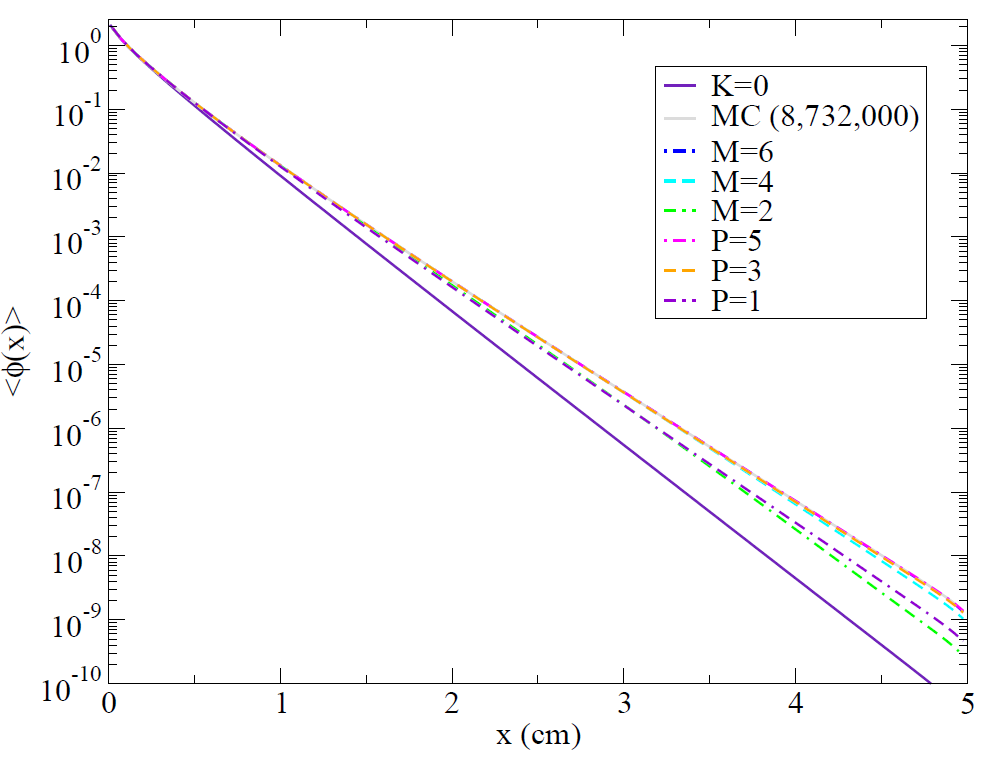
\includegraphics[width=\textwidth]{FichtlScalarMean_c0_5.PNG}
    \caption{}
    \label{fig:FP:parta}
  \end{subfigure}
  \begin{subfigure}[b]{0.475\textwidth}
    \centering
    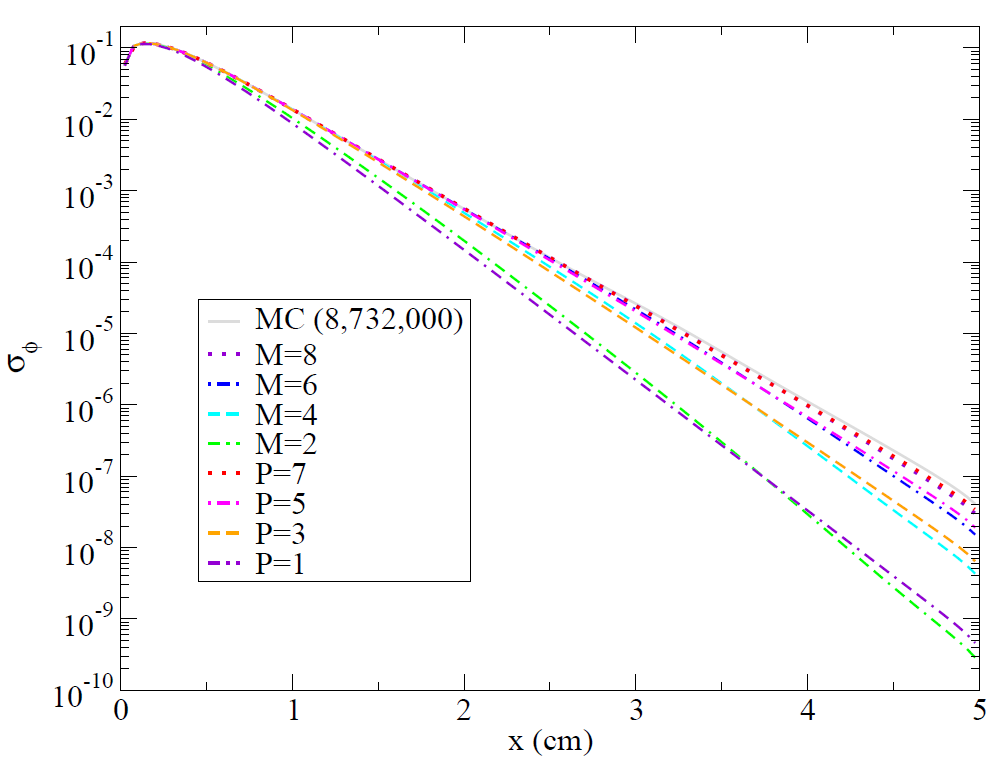
\includegraphics[width=\textwidth]{FichtlScalarDev_c0_5.PNG}
    \caption{}
    \label{fig:FP:partb}
  \end{subfigure}
  %
  \begin{subfigure}[b]{0.475\textwidth}
    \centering
    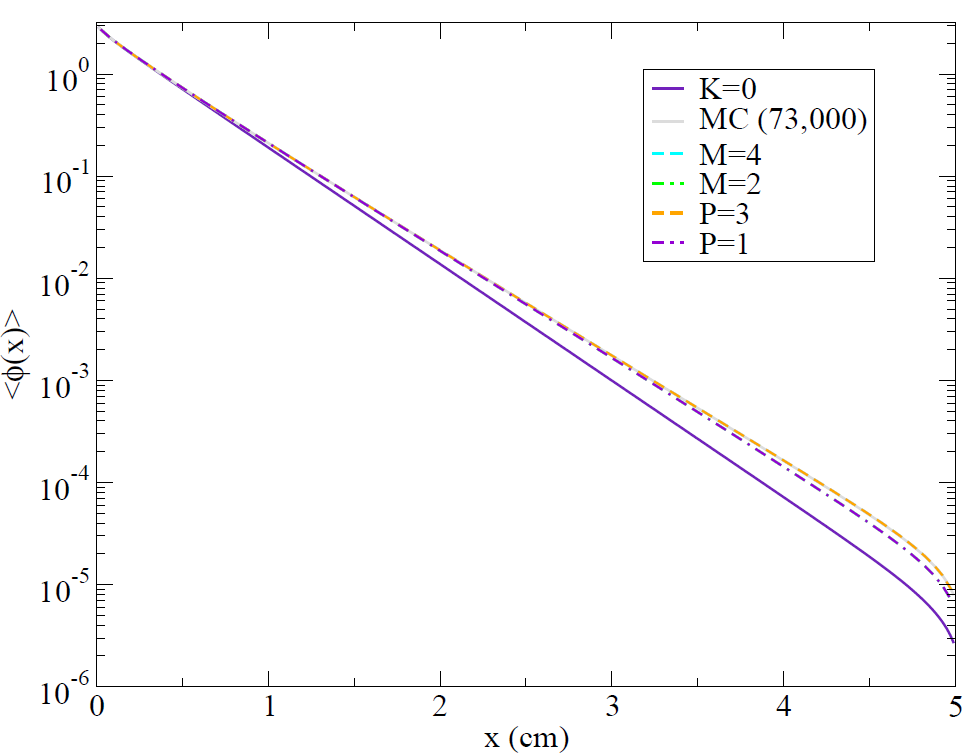
\includegraphics[width=\textwidth]{FichtlScalarMean_c0_9.PNG}
    \caption{}
    \label{fig:FP:partc}
  \end{subfigure}
  \begin{subfigure}[b]{0.475\textwidth}
    \centering
    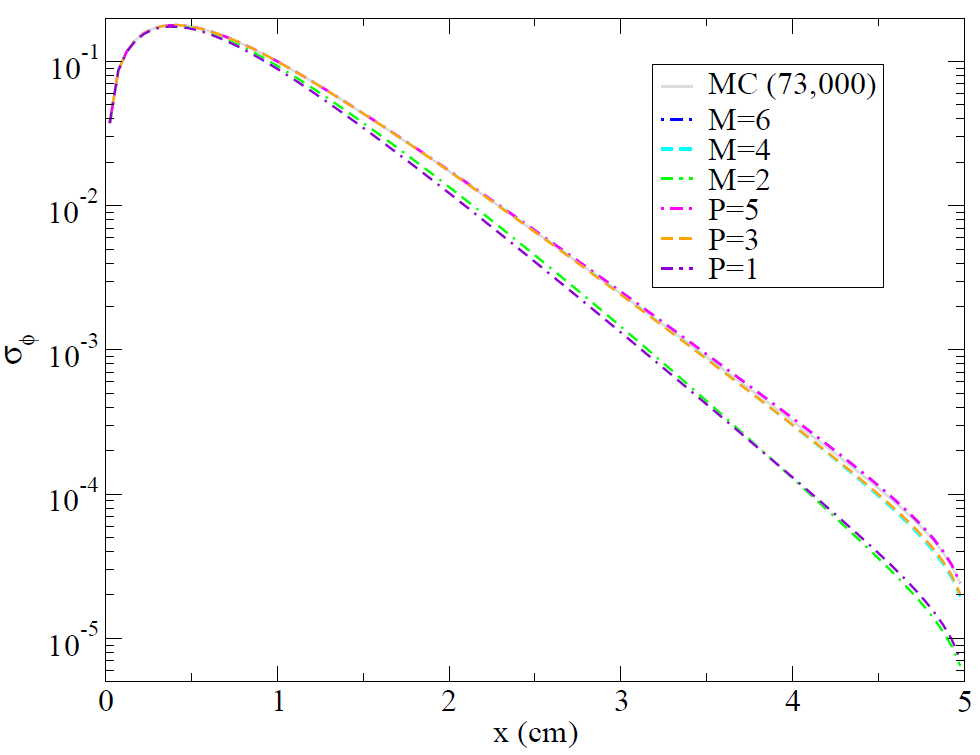
\includegraphics[width=\textwidth]{FichtlScalarDev_c0_9.PNG}
    \caption{}
    \label{fig:FP:partd}
  \end{subfigure}
  \caption{Flux mean and standard deviation (dev) as a function of length through a slab for two different problems defined by the value of input parameter $c$: \protect\subref{fig:FP:parta} flux mean, $c = 0.5$; \protect\subref{fig:FP:partb} flux dev, $c = 0.5$; \protect\subref{fig:FP:partc} flux mean, $c = 0.9$; \protect\subref{fig:FP:partd} flux dev, $c = 0.9$.}
  \label{fig:FluxPlots}
\end{figure}

Figure~\ref{fig:AMClosure} is a screenshot of a figure from Ref.~\cite{PautzSAND2017AMClosurePres} and serves as an example of one-column figures.
Figure~\ref{fig:DonovanFig1} is a screenshot of Figure 1 in an NSE article~\cite{DonovanNSE2003}, uses the caption given in that paper, and serves as an example of two-column figures.
Figure~\ref{fig:FluxPlots} contains four related plots from Ref.~\cite{Fichtl2009dissertation} of scalar flux average or standard deviation for each of two different problems defined by the value of scattering ratio $c$.
Figures may have multiple parts.
In this case, each part should be labeled and referenced with~\subref{fig:FP:parta}, \subref{fig:FP:partb}, etc., instead of directional descriptions (e.g. `left,' `right,' `upper-left,' etc.).
The figure caption should discuss each part following the part label as in Figure~\ref{fig:FluxPlots}.


\section{Sections}
\label{sec:sections}

You will likely want to use subsections to keep the paper organized and easy to read.

\subsection{Example 1 of B-level Heading}

Subsections are formatted in this way.

\subsection{Example 2 of B-level Heading}

If you have one subsection, ideally you should have at least two.

\subsubsection{Example 1 of C-level Heading}

Subsubsections may also be used.

\subsubsection{Example 2 of C-level Heading}

But again, it is preferred to have at least two.



\section{Conclusion}
\label{sec:conclusion}

We hope this template serves you well.
For the current information on ANS document formatting, visit \url{http://www.ans.org/pubs/journals/nse/authors/} for the NSE journal or the equivalent sites for the \href{http://www.ans.org/pubs/journals/nt/authors/}{NT} and \href{http://www.ans.org/pubs/journals/fst/authors/}{FST} journals.



\pagebreak
\section*{Acknowledgments}

Template creation supported by the Department of Energy Computational Science Graduate Fellowship, provided under grant number DE-FG02-97ER25308.



\pagebreak
\bibliographystyle{ans_js}                                                                           %custom ANS journal submission template bibliography style
\bibliography{bibliography}

%%% If you desire to place footnotes at the end of the document, uncomment these two lines and the four related near the beginning of this file
%\pagebreak
%\theendnotes

\end{document}


